\documentclass[11pt,a4paper]{article}
% What we did since the call of 25 September 2026, explained from scratch.
% Every number is read from a registered output (experiments/registry/E*.json and the frozen files it lists);
% the few exceptions are flagged in the text. Checked claim by claim against the frozen files on 9-10 Oct 2026.
\usepackage[T1]{fontenc}
\usepackage[utf8]{inputenc}
\usepackage{newtxtext,newtxmath}
\usepackage[margin=2.1cm]{geometry}
\usepackage{microtype}
\usepackage{booktabs}
\usepackage{array}
\usepackage{tabularx}
\usepackage{graphicx}
\usepackage{float}
\usepackage[font=small,labelfont=bf]{caption}
\usepackage{xcolor}
\usepackage{enumitem}
\usepackage{tikz}
\usetikzlibrary{arrows.meta,positioning,calc}
\usepackage[hyphens]{url}
\usepackage[hidelinks]{hyperref}
\graphicspath{{figures/}}
\setlist{itemsep=0.12em,topsep=0.25em,leftmargin=1.2em}
\definecolor{ink}{HTML}{1F2937}
\definecolor{acc}{HTML}{2563EB}
\definecolor{soft}{HTML}{EFF4FB}
\newcommand{\key}[1]{\par\smallskip\noindent\colorbox{soft}{\parbox{\dimexpr\linewidth-2\fboxsep}{\small\textbf{In one line.} #1}}\par\smallskip}
\newcommand{\src}[1]{{\footnotesize\color{gray}[#1]}}
\newcommand{\fals}[1]{{\small\itshape #1}}
\newcolumntype{L}{>{\raggedright\arraybackslash}X}
\setlength{\parskip}{0.35em}
\renewcommand{\topfraction}{0.9}\renewcommand{\bottomfraction}{0.8}\renewcommand{\textfraction}{0.07}
\renewcommand{\floatpagefraction}{0.85}\setcounter{topnumber}{3}\setcounter{totalnumber}{4}
\setlength{\parindent}{0pt}

\title{\textbf{What we did since the call of 25 September}\\[0.3em]\large What to know before writing to Jérôme, then an explanation from scratch}
\author{Prepared for Giovanni Mantovani}
\date{14 October 2026}

\begin{document}
\maketitle
\vspace{-1.6em}

\begin{abstract}\noindent
The first two pages are what you need before replying. The rest explains the work from scratch and can be read in any order:
\textbf{Part I} answers the eleven questions Jérôme asked on 25 September, \textbf{Part II} is the $\phi^4$ field he and Marc proposed
afterwards. Every number comes from a run registered in advance with its output frozen by a checksum (the few exceptions are
flagged); a prediction that turned out wrong is reported in \fals{italics}: a falsified prediction is a result, not a failure.
\end{abstract}



%=====================================================================================================
\section*{Before you write to Jérôme}

\textbf{What happened since the call.} (1) His eleven questions were answered with experiments written down before they ran
(table below). (2) The second laboratory he and Marc proposed, snapshots of the $\phi^4$ (stochastic Allen--Cahn) field, was built
and run: six settings, five estimators and an exact reference. (3) We tested where the method stops: a hidden variable shared by a
whole sequence, subsampled chains, a chain outside the kernel family, data out of equilibrium. (4) BP was made cheaper (a coarser
grid) and the ``speciation'' experiment he suggested was run. (5) On 12 October the \emph{paper was rewritten} to follow the
structure of their note of 30 September; the draft is waiting for your approval.

{\small
\begin{tabularx}{\linewidth}{@{}l>{\raggedright\arraybackslash}p{0.27\linewidth}L@{}}
\toprule
 & Jérôme's question & Answer in one line \\
\midrule
Q1 & Gaussian messages = Gaussian score = Kalman smoother? & Yes, proved and checked to $2\times10^{-13}$. \emph{Not new:} the thesis already had it; the
 paper just never said ``Kalman''. Forcing messages Gaussian on a grid fails numerically (error up to 0.26). \\
Q2 & Is BP exact with a Laplace-like message family? & No: exact at the first site only; fails in the interior in 432 of 432 configurations. \\
Q3 & What do the messages look like? & Very close to his guess (a Gaussian passed once through the kernel): KL $2{,}272\times$ below a plain Gaussian's. \\
Q4 & Can any finite family close the recursion? & The Gaussian does; his family does not; no proof for other families. \\
Q5 & BP in Fourier space? & Not worth building: partly works as a representation, unreliably; our FFT solver is $5.8\times$ \emph{slower}. \\
Q6 & Neural network as the kernel? & Loses on the paper's chain (64 of 64 comparisons) but wins where the simple family is wrong (below). \\
Q7 & Time per sequence, network vs BP? & BP is slower: $12.5\times$ the largest transformer on 8 threads, $3.2\times$ on one thread. A coarser grid cuts BP by 4--6$\times$. \\
Q8 & Sample without diffusion? & Yes, exactly, and $731\times$ cheaper than a 200-step reverse process. \\
Q9 & Error at fixed $t$ or pooled? & Per level: EM--BP beats every network at all 12 levels and the Gaussian score at the 8 ($M=128$) or 10 ($M=2048$) lowest. \\
Q10 & Information curves: $\rho,\beta$ or $\kappa_2,\kappa_4$? & Recomputed in cumulant coordinates; the message survives (fourth order falls about $700\times$ more than second). \\
Q11 & How does the cost scale in $M$ and $L$? & Linearly in both; in the grid like $N_g^{1.2}$, not $N_g^{2}$ (the call's answer was wrong). \\
\bottomrule
\end{tabularx}}

\textbf{The four results that carry the story.}
\begin{enumerate}[leftmargin=1.6em]
\item \emph{The paper's chain.} A 25-number kernel learned from one noisy copy of each sequence, inside exact BP, beats every neural
denoiser at every noise level and sample size, although the networks are trained on the clean sequences ($M=2048$: error 0.023
against 0.060 for the best network).
\item \emph{The $\phi^4$ field.} The paper's own kernel (a linear drift) fails there: it does no better than the linear baseline.
The field's own 5-number form, a Gaussian bond plus a quartic potential per site, is best on every setting: 3--17\% of the linear
baseline's error, and the best network is 14--24 times worse. Samples from it have the right kinks and domain lengths, and its fitted
temperature is within 10\% of the truth in 96 of 96 fits.
\item \emph{The kernel family is the modelling choice.} A flexible (neural) kernel earns its parameters only when the simple
family is wrong: on a chain with a sharp Laplace bond it is 1.8--2.5 times better, and on a chain subsampled every fourth site it is
below the site energy in 16 of 16 seeds; where the simple family is right it loses.
\item \emph{What exact inference costs.} BP is slower per sequence than a network, and the paper says so; the cheap lever is the grid
(101 points suffice for the $\phi^4$ kernels), not Fourier modes.
\end{enumerate}

\textbf{Where Jérôme may push, and what we did not show.}
\begin{itemize}
\item The comparison with networks equalises the data, not the algorithm: the networks timed are the largest variants and in Part I they
see clean sequences (they get more than EM--BP). The paper does not claim to rank learning algorithms.
\item Several network-kernel results are upper bounds: the fit was still improving when its budget ended, so the true risk is lower.
\item Speciation: commitment time behaves as predicted, but our prediction for the kink-energy law failed (fit 0.988 against
$2\sqrt2/3\approx0.943$, within 2\% predicted), so we do not claim the asymptotic constant; in one dimension there is no phase transition.
\item A hidden variable shared by the whole sequence leaves a bias that no amount of data removes; augmenting the state repairs it.
\item Some of our predictions were wrong and are reported as such (italics below). Three runs of 26 September were frozen after
being read, which the registry says openly; an audit on 9 October re-derived the numbers and changed no verdict.
\end{itemize}

\textbf{Waiting for you before you reply} (details in Section~4): the framing (a general Markov kernel, the linear chain first and the
field second, the field in the body) and the figure choice are drafted, not decided; the Milan date; and Marc should be on the reply.

\bigskip
\key{The paper's claim, in plain words. A diffusion model needs, at every noise level, the best guess of the clean data given the
noisy data. When the data are a Markov chain (each value depends only on the previous one), that guess can be computed
\emph{exactly} from a small model of one step of the chain, and the one-step model can be learned from noisy data alone. Done this
way it beats neural denoisers trained on the same sequences, even when the networks see them clean, \emph{provided} the one-step
model has the right form: on the physical field of Part II the paper's original form fails and the field's own form wins.}

%=====================================================================================================
\section{The method from zero}

\textbf{The data.} Sequences $a_1,\dots,a_L$ that form a \emph{Markov chain}: given $a_i$, the next value $a_{i+1}$ does not depend
on anything earlier. The law is then fixed by the \emph{transition kernel} $K(a'\mid a)$, the density of the next value given the
current one (plus the law of the first site, which for a stationary chain follows from $K$). The paper's test chain is
\emph{linear}: $a_{i+1}=\rho\,a_i+\varepsilon_i$ with non-Gaussian (Laplace) driving noise $\varepsilon_i$.

\textbf{What a diffusion model needs.} It corrupts the data at a level $t$, $x=e^{-t}a+\sqrt{\Delta_t}\,z$ with $\Delta_t=1-e^{-2t}$ and
$z$ standard Gaussian noise, and learns the \emph{score} $\nabla_x\log p_t(x)$, where $p_t$ is the density of the corrupted $x$. The
score is used to denoise and, run backwards from pure noise (the ``reverse process''), to generate. By Tweedie's identity
\[
\nabla_x\log p_t(x) \;=\; -\,\frac{x-e^{-t}\,\mathbb E[a\mid x]}{\Delta_t},
\]
so the score is equivalent to the best denoiser in mean squared error, the posterior mean $\mathbb E[a\mid x]$.

\textbf{Why a chain is special.} On a chain the posterior mean can be computed exactly by \emph{belief propagation} (BP), the
forward--backward algorithm: one sweep left to right and one right to left, each carrying a ``message'' (a function over one
site's value) through $K$. We store each message on a grid of 401 points on $[-8,8]$ (``grid BP''). With the true kernel this
gives the reference score, accurate to the grid's quadrature error; we call it the \textbf{oracle}.

\textbf{When the kernel is unknown} we learn it from the noisy sequences by \emph{EM} (expectation--maximisation): with the
current $K$, run BP on each noisy sequence to get the posterior of every neighbouring pair (E-step); refit $K$ to those soft pair
counts (M-step); repeat. ``EM--BP'' is this, followed by BP with the learned kernel.

\begin{figure}[!htbp]\centering
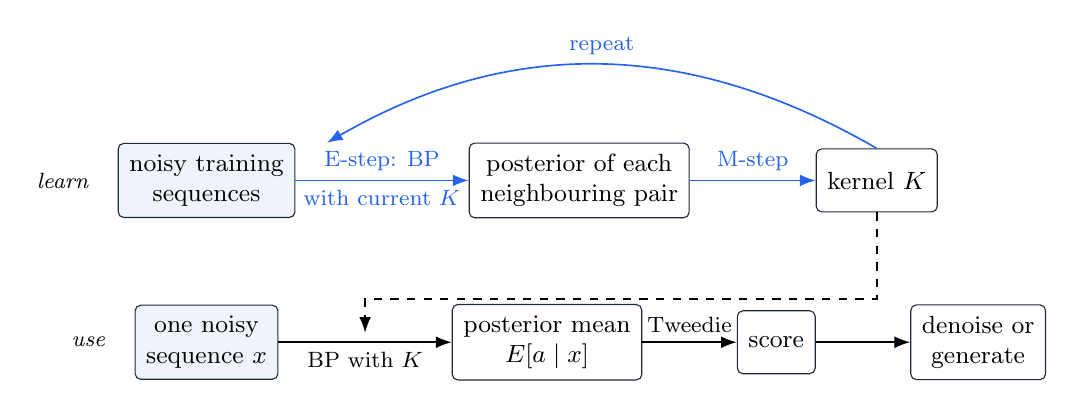
\begin{tikzpicture}[font=\small,
  box/.style={draw=ink, rounded corners=2pt, inner sep=4pt, minimum height=8mm, align=center},
  arr/.style={-{Latex[length=2mm]}, line width=0.6pt}]
  \node[box, fill=soft] (d) {noisy training\\sequences};
  \node[box, right=2.2cm of d] (p) {posterior of each\\neighbouring pair};
  \node[box, right=1.6cm of p] (k) {kernel $K$};
  \draw[arr, acc] (d) -- node[above, font=\footnotesize]{E-step: BP} node[below, font=\footnotesize]{with current $K$} (p);
  \draw[arr, acc] (p) -- node[above, font=\footnotesize]{M-step} (k);
  \draw[arr, acc] (k.north) to[out=150, in=30] node[above, font=\footnotesize]{repeat} ($(d.north east)+(0.4,0)$);
  \node[box, fill=soft, below=1.1cm of d] (x) {one noisy\\sequence $x$};
  \node[box, right=2.2cm of x] (m) {posterior mean\\$\mathbb E[a\mid x]$};
  \node[box, right=1.2cm of m] (s) {score};
  \node[box, right=1.2cm of s] (g) {denoise or\\generate};
  \draw[arr] (x) -- node[below, font=\footnotesize]{BP with $K$} (m);
  \draw[arr] (m) -- node[above, font=\footnotesize]{Tweedie} (s);
  \draw[arr] (s) -- (g);
  \draw[arr, dashed] (k.south) |- ($($(x.east)!0.5!(m.west)$)+(0,0.55)$) -- ($($(x.east)!0.5!(m.west)$)+(0,0.12)$);
  \node[left=0.25cm of d, font=\footnotesize\itshape] {learn};
  \node[left=0.25cm of x, font=\footnotesize\itshape] {use};
\end{tikzpicture}
\caption{The method. Top: EM learns the kernel from noisy data, with BP inside. Bottom: BP with the learned kernel gives the
posterior mean and hence the score. A neural denoiser learns the map from $x$ to the posterior mean (or score) directly instead.}
\end{figure}

\textbf{The kernels} we fit inside EM--BP (one table for the whole document):

\begin{table}[!htbp]\centering\small
\caption{Kernel families. The middle three are one model class (a Gaussian step re-weighted by a function of where it lands).}
\label{tab:kernels}
\begin{tabularx}{\textwidth}{@{}l L r@{}}
\toprule
name & what it is & numbers \\
\midrule
mixture (the paper's kernel) & next value $=\rho\times$ current $+$ noise drawn from an 8-component Gaussian mixture: the expected next value is \emph{linear} in the current one & 25 \\
tilted spline & a Gaussian step re-weighted by a smooth function $w(a')$ of the landing point ($\log w$ a spline) & 25 \\
Legendre tilt & the same, $\log w$ a polynomial & 7 \\
site energy & the field's own form (Jérôme's pair energy): a Gaussian ``bond'' between neighbours plus a quartic potential at each site & 5 \\
unrestricted & $\log K$ any smooth function of $(a,a')$ (a $10\times10$ spline); assumes no Gaussian bond & 100 \\
MDN & a mixture density network: a small neural net mapping $a$ to a Gaussian mixture for $a'$ & 1{,}516 \\
\bottomrule
\end{tabularx}
\end{table}

\textbf{The competitors.} (i) \emph{Neural denoisers} (window CNN, transformer, bidirectional GRU, TCN, U-Net, MLP) trained on the
same $M$ sequences. In Part I they see the sequences \emph{clean} and are corrupted afresh at every training step (denoising score
matching), so they get strictly more than EM--BP, which sees one noisy copy of each. In Part II they are trained both ways: on one
noisy copy (``ISM'', EM--BP's own setting) and on clean targets with one fixed corruption (``DSM''). (ii) The \textbf{linear baseline} (called the ``linear floor'' in the reports): the best \emph{linear} denoiser,
built from the true covariance. On a linear chain, Gaussian closure of BP (forcing every message to be Gaussian) returns exactly
this (the paper's Proposition~1). A method that goes \emph{below} it uses structure beyond second order. In this document
``Gaussian'' methods always mean this baseline unless said otherwise.

\textbf{How a method is scored.} Its \emph{risk} is a relative RMS error,
\[ R=\Big(\textstyle\sum\|\hat S-S\|^2\big/\sum\|S\|^2\Big)^{1/2}, \]
with $\hat S$ its score, $S$ the oracle score, and the sums over test chains, sites and twelve noise levels $t$ from $0.05$ to $3$.
$R=0$ is perfect and a zero score has $R=1$. Because it pools sums, the low-noise levels dominate (the six lowest carry 98--99.5\% of
the squared error for EM--BP and the linear baseline, 88--95\% for the networks). $M$ is the number of training sequences; a
\emph{seed} is an independent repetition with fresh data and initialisation. For EM--BP and the networks alike, the stopping point is
chosen on a validation set by this oracle risk. An oracle-free rule for EM (held-out likelihood) is also recorded: on the paper's
chain it picks the same stopping point (7 of 8 settings); on the field it gives somewhat larger risks (Section~3.3).

\textbf{How the work is kept honest.} Experiments since 25 September (E22, E23, \dots) have a registry file written before the main
run, with predictions and the script that will read them; amendments are dated in the file. Outputs are frozen by checksum (three
runs of 26 September were frozen late, on 9 October, after being read). A prediction is read by its own rule: CONFIRMED,
FALSIFIED, or UNRESOLVED when the rule cannot decide (for example a model still improving when its budget ran out).



%=====================================================================================================
\section{Part I: Jérôme's eleven questions (call of 25 September)}

The test model is the paper's linear chain with $\rho=0.85$, Laplace (sharp-peaked) driving noise and $L=32$ sites, unless a
question needed another (stated). The questions fall into five themes.

\textbf{A. Can BP's messages be summarised by a few numbers?} (Q1--Q5). This matters because the 401-point grid is where BP
spends its time: a parametric family that BP maps onto itself (a ``closed'' family) would replace the grid.
\begin{itemize}
\item \textbf{Q1. Gaussian messages = Gaussian score = Kalman smoother?} Yes on a linear chain: the paper's Proposition~1 proves that
BP with Gaussian messages returns the best linear denoiser. As a numerical check, on a Gaussian chain the exact score computed three
ways (closed form; an independent Kalman smoother, i.e.\ the Rauch--Tung--Striebel forward--backward filter; our grid BP) agrees to a
relative error of $1.9\times10^{-13}$. \fals{A registered clause failed: BP with messages forced to be Gaussian, run on the same
401-point grid, was off by up to 0.26 in relative score error, because its backward messages widen beyond the grid's edge.} \src{E39}
\item \textbf{Q2. With Laplace noise, is BP exact with a Laplace-like message family?} No. We tested Jérôme's family (a Gaussian passed
once through the kernel) and a Gaussian+Laplace mixture. Jérôme's family is exact at the first site only (error at machine precision); deeper in the chain
its error, the KL divergence to the true message, is about $1.6\times10^{-5}$ at site 31 at low noise, small but not zero, so BP with
it is not exact. \src{E22}
\item \textbf{Q3. What do the messages look like?} Close to Jérôme's family: at low noise its KL to the true message is $2{,}272\times$
smaller than a plain Gaussian's and $78\times$ smaller than the 4-parameter Gaussian+Laplace mixture's. \fals{We predicted it would do best at high
noise; it does worst there, and the mixture overtakes it.} \src{E22}
\item \textbf{Q4. Can any finite family close the recursion?} The Gaussian does (on a Gaussian chain). Jérôme's family does not (in
432 of 432 configurations). We have no proof that no other finite family closes; approximately (refit after each step) any
family works, at a measured price. \src{E22}
\item \textbf{Q5. BP in Fourier space with $\sim$20 modes (Fourier coefficients)?} As a \emph{representation}, partly: on the Laplace
chain a Fourier basis on a window adapted to each message needs 33 numbers (KL $10^{-2}$) or 47 ($10^{-4}$) against the grid's 45
and 151, but it reaches $10^{-4}$ in only 53 of 144 cases and adding modes can make it worse, so a solver could not choose a
truncation and know its error. Merely speeding up the transition step on the grid (by FFT) is capped at about $1.15\times$, because
that step is 12--15\% of a BP sweep; an FFT version we built is second-order accurate ($6.7\times10^{-4}$ from dense BP) but $5.8\times$ slower at 401 points. The cheap lever
turned out to be a coarser grid (Section~3.6). \src{E23, E24x, E40}
\end{itemize}

\textbf{B. Can the kernel be a neural network?} (Q6). It can be fitted by EM, and it loses: the MDN is worse than the 25-number
mixture kernel in 64 of 64 comparisons (median factor 2.0--2.5), and also worse than the best plain score network (which has
19--25\% lower risk). \fals{We predicted it would sit between the networks and EM--BP.} With 61 times more parameters it does 2--2.5 times worse on test data, consistent with the overfitting Jérôme expected. This verdict is for the paper's chain, where a small kernel is
correctly specified; where it is not, the network kernel does win (Section~3.4). \src{E25m, E30}

\textbf{C. Cost} (Q7, Q11). BP is slower per sequence; by how much depends on threads and grid size. On the paper's 401-point grid
with 8 threads BP takes 0.52\,ms per sequence against 0.042\,ms for the transformer ($12.5\times$); on an H200 GPU $15\times$ at
batch 512 and $6\times$ at batch 2048. With one thread the gap narrows, because the networks use threads and BP barely does: at
401 points BP is 3.2 times slower than the transformer and 10.6 times slower than the GRU; at 151 points (0.173\,ms) it is faster
than the transformer and TCN but still 2.7 times slower than the GRU and 7 times slower than the window network. (The networks timed are
the largest screened variants, several times the size of those scored.) Cost grows linearly with the number of sequences and with $L$; the grid enters
like $N_g^{1.2}$, not $N_g^2$, because elementwise work dominates. \src{E24x, E47}

\textbf{D. Sampling without diffusion} (Q8). Yes: drawing site 1 and then each next site from the true kernel (ordinary Markov-chain
simulation) samples exactly. We compare samplers by the KL divergence between their residual histograms and a large reference
sample: exact simulation sits at the Monte Carlo floor, the reverse process with the exact score needs 200 steps to get there, and
exact simulation is $731\times$ cheaper (8 threads, 2,048 sequences). With a fitted kernel the samples inherit the kernel's error, the same as the reverse process gives. A Gaussian score
generates Gaussian samples: the excess kurtosis of the residual $a_{i+1}-0.85a_i$ is about 0 against 1.92 for exact samples at the same final noise
level (descriptive, no prediction). \src{E27, E26}

\textbf{E. How we evaluate} (Q9, Q10). Q9: per noise level, EM--BP beats every network at all 12 levels. It beats the linear
baseline (which knows the true covariance) at the 8 (with $M=128$) or 10 ($M=2048$) lowest levels; above that the remaining
non-Gaussian structure is smaller than the fitted kernel's estimation error, and the crossover moves up with data. \fals{We
predicted EM--BP would be first at every level.} \src{E28}
Q10: a panel of the paper plots, against $t$, how much information the noisy data carry about the chain's correlation (a
second-order property) and about the shape of its noise (fourth order). Jérôme asked whether the shape curve measures the fourth
cumulant $\kappa_4$ or the parameter $\beta$ of the noise law. Recomputed for $\kappa_4$, the ratio of fourth- to second-order information falls from 0.071 at $t=0.05$ to $9.9\times10^{-5}$ at
$t=3$, a factor of about $700$, so the paper's message survives (the figure script recomputes it in memory from the frozen E01 file;
the derived table itself is not frozen; an earlier figure of $164\times$ used $t=4$, where the estimator sits at its numerical
floor). The old panel plotted $\beta$ under the label ``fourth order'', which is off from the $\kappa_4$ curve by 1.6--1526$\times$;
the rewritten draft re-plots it in cumulant coordinates (Section~4).

\fals{Other registered Part I predictions that failed, all reported in the registry: the grid exponent of 2 (it is 1.2), a
representation beating the grid by at most $4\times$ (Fourier on adapted windows does better, unreliably), one exact sweep beating
the reverse process on kurtosis (they tie at the Monte Carlo floor), and the FFT breaking even at 3,201 points.}

\key{On the paper's test model, EM--BP with a 25-number kernel, learned from one noisy copy of each sequence, beats every network
(trained on the clean sequences) at every noise level; exact sampling needs no diffusion; per sequence BP is slower than the
networks, by $12\times$ on many threads and by 1--3$\times$ against the larger networks on one thread with a coarser grid.}

%=====================================================================================================
\section{Part II: the $\phi^4$ field}

\subsection{The model}

Think of a one-dimensional elastic string whose height $\phi(s)$ at position $s$ prefers the values $+1$ or $-1$, shaken by thermal
noise at temperature $\Theta$. Its energy is $H[\phi]=\int\big(\tfrac12\phi'(s)^2+V(\phi(s))\big)\,ds$ with the double well
$V(\phi)=(\phi^2-1)^2/4$, and its dynamics is the stochastic Allen--Cahn equation
$\partial_\tau\phi=\partial_s^2\phi-V'(\phi)+\sqrt{2\Theta}\,\eta$ ($\tau$ is physical time, $\eta$ space--time white noise). It settles into the Gibbs
law $\propto e^{-H[\phi]/\Theta}$. A snapshot (Figure~\ref{fig:field}) shows \emph{domains} near $+1$ and $-1$ separated by
\emph{kinks}; the energy of one kink is $E_{\rm kink}=2\sqrt2/3\approx0.94$. When cold, domains are long and the values have a
two-humped histogram.

\begin{figure}[!htbp]\centering
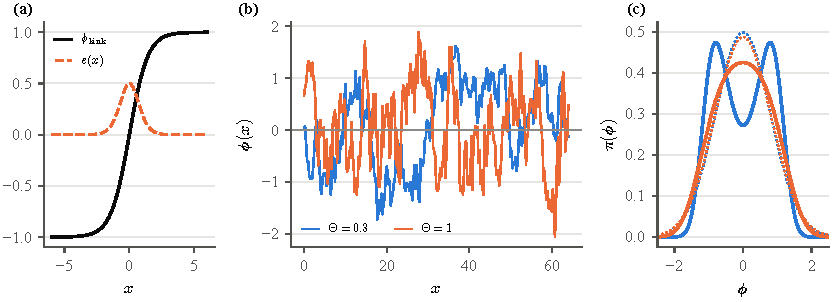
\includegraphics[width=\textwidth]{primer-field.pdf}
\caption{(a) One kink, the field crossing from $-1$ to $+1$, and its energy density. (b) Two exact snapshots on a lattice of
spacing $h=0.25$, at $\Theta=0.3$ (long domains) and $\Theta=1$. (c) The exact density of the field values (solid) against a Gaussian
of the same variance (dotted), $h=0.25$: two humps when cold.}
\label{fig:field}
\end{figure}

\textbf{Why it fits the method exactly.} On a lattice of spacing $h$ the energy only couples neighbouring sites:
\[ H_h=h\textstyle\sum_i\big[\tfrac12\big((\phi_{i+1}-\phi_i)/h\big)^2+V(\phi_i)\big], \]
so the Gibbs law factorises along the lattice, and a snapshot
$\phi_1,\dots,\phi_L$ is \emph{exactly} a Markov chain in the site index, and its kernel is a Gaussian step of variance $\Theta h$ re-weighted by a function of where it lands (a
``tilted walk''; Table~\ref{tab:kernels}). The site energy contains the truth exactly; the spline and Legendre tilts are flexible
members of the same class. Unlike the paper's linear chain, the expected next value is a non-linear function of the current one
(on cold cells it pushes sites off the barrier at 0 towards the domain values), so the mixture kernel, which is linear in this
sense, cannot represent it.
The \emph{correlation length} $\xi$ (over how many sites correlations decay by a factor $e$) grows fast as $\Theta$ falls.

\textbf{Six test settings (``cells'').}

\begin{table}[!htbp]\centering\small
\caption{The cells, and the risk of two reference methods. The iso cells have $h$ chosen so that the slowest correlation mode
decays at the same rate as the base cell's (correlation length about 6 sites). The last row ignores both the neighbours and the
two humps (it shrinks each value towards 0).}
\label{tab:cells}
\begin{tabular}{@{}lcccccc@{}}
\toprule
 & base & iso & iso & iso & finer & finest \\
temperature $\Theta$ & 0.3 & 0.5 & 1 & 2 & 0.3 & 0.3 \\
spacing $h$ & 1 & 0.42 & 0.23 & 0.15 & 0.5 & 0.25 \\
sites $L$ & 32 & 32 & 32 & 32 & 64 & 128 \\
\midrule
linear baseline & 0.269 & 0.115 & 0.058 & 0.041 & 0.162 & 0.098 \\
each site alone with a Gaussian prior & 0.674 & 0.657 & 0.657 & 0.656 & 0.714 & 0.750 \\
\bottomrule
\end{tabular}
\end{table}

The linear baseline measures how much there is to gain beyond a Gaussian model at each cell. It falls with temperature, and also
under refinement, where the histogram stays nearly as two-humped (excess kurtosis $-1.35$ to $-1.22$) but neighbouring sites
become more redundant. \src{E32}

\subsection{Checking the instruments}

\begin{itemize}
\item \textbf{The oracle is exact}: on every cell grid BP at 401 points agrees with a four-times finer grid to $1.3\times10^{-12}$
(checked before any learning). Later, on a Gaussian chain, grid BP matched two independent exact answers to $1.9\times10^{-13}$.
\src{E32, E39}
\item \textbf{Forcing BP's messages to be Gaussian breaks down on the field}: the backward messages become almost flat and their mass
piles up at the grid edge. So the Gaussian comparison is the linear baseline itself, computed in closed form. \src{E32}
\item \textbf{The paper's information-decay theorem} (Theorem~5 in the rewritten draft: the squared gap to the Gaussian score is a known
constant times $e^{-8t}$ at large $t$) is not reached within the schedule: the measured/predicted ratio at $t=3$ is 0.85, 0.86, 0.73,
0.94 on the four $L=32$ cells, and on the $\Theta=1$ cell it falls over the last step. \fals{Registered as ``approaches 1'': unresolved.}
\src{E32}
\item \textbf{Cost} (measured on the paper's chain; BP's cost does not depend on the model): one BP call on 512 sequences of 32 sites
needs about 260\,MB, five message-sized arrays, linear in everything, 1.8--4.2 times the largest network. \src{E38}
\end{itemize}

\subsection{Learning the kernel through noise: the main result}

Each training sequence enters as one noisy copy at one of the twelve noise levels. EM--BP and the ISM networks never see clean
data; the DSM networks also get the clean targets, which favours them, and still lose.
\begin{itemize}
\item \textbf{The 5-number site energy is the best method on every cell at every size} (on average over seeds). At $M=2048$ its risk is
3--17\% of the linear baseline (4--23\% with the oracle-free stopping rule) and 43--59\% below the spline; it reads the temperature off
the noisy data within 10\% in 96 of 96 fits. With very little data on the two hottest cells it still loses to the baseline ($M=32$: $1.4\times$); from
$M=128$ it wins on every cell on average (16 of 16 seeds from $M=512$). \fals{We had predicted it would be within 10\% of the
spline; it is far better.}
\item \textbf{The paper's own mixture kernel learns nothing beyond the linear baseline} (1.00--1.02 times it at $M=2048$): a kernel whose
expected next value is linear cannot hold sites in a domain. On non-linear physics the kernel family matters.
\item \textbf{Networks lose to the spline and the site energy on every cell}: 4--27 times the spline's risk, and above the linear
baseline on the hot cells (on the cold cells they do beat the paper's mixture kernel). The window network chose its radius per cell from $\{2,4,8\}$ sites and picked 2, 4, 8 at $h=1,\tfrac12,\tfrac14$, a constant
physical reach (at $h=\tfrac14$ the largest offered). Its absolute risk fell (0.149 to 0.118) but relative to the baseline it rose from
0.55 to 1.20 (ISM version): Jérôme's expectation that structure gains under refinement holds, even though the window was free to
widen with the lattice. \fals{We had predicted its absolute risk would
grow.} Whether an even wider window closes the gap was not tested.
\item \textbf{The good kernels are physically right}: samples drawn from the spline and the site energy reproduce the kink density and
mean domain length within a few per cent, and the whole distribution of domain lengths within 10\% at every quantile,
statistically indistinguishable from exact samples (4 seeds; one quantile is 10.4\% off). On the three cold cells the mixture's
samples have about 1.4 times too many kinks and domains 12--18\% too short at the median; on the hotter cells they are within
about 10\%.
\item \textbf{Two doubts removed.} The MDN's gap to the spline (1.9--4.3$\times$) is not a training-budget artefact: four times the EM budget lowers its risk by only
0.4--4.5\% (\fals{we predicted more than 10\%}). The potential's barrier height is learnable at high temperature, just slowly: at
$\Theta=2$ its error falls like $M^{-0.54}$ and all 16 seeds are within 20\% at $M=32{,}768$.
\end{itemize}
\fals{Other registered predictions that failed here. Two on substance: with little data at high temperature ($M=128$, $\Theta=2$)
the paper's mixture beats the spline in 12 of 16 seeds, and the 7-number Legendre tilt crashes numerically on the finest lattice
(39 fits); the raw count of sign changes is not a lattice-independent kink density (a coarse count replaced it). The rest on
thresholds set too tight: the barrier at $\Theta=1$ (14 of 16 seeds within 20\%, not 16), the domain-length KS test, the tail
deficit of the mixture's domains.}
\src{E33, E34, E37, E41, E42}

\key{With the right kernel family, exact BP using a kernel learned from noisy data beats the linear baseline and every network by a
wide margin on real non-linear physics; with the paper's linear-drift mixture it collapses to the Gaussian answer.}

\subsection{When the assumptions break}

\textbf{A hidden variable shared by the whole sequence} (on a Gaussian test chain with a closed-form answer, not the field). Each
sequence is $b\,G+U$, with $U$ a Gaussian linear chain ($\rho=0.85$) and $G=\pm1$ a hidden sign per sequence; the data are no longer Markov. The paper's
first-order kernel (it conditions on one previous site) gets stuck: at $b=2$ four times more data change its risk by $+0.2\%$, and at
$M=2048$ it is 1.57 ($b=2$) and 1.67 ($b=1$) times \emph{worse} than the linear baseline, in 16 of 16 seeds. Running BP on pairs
(value, sign), so that it also infers each sequence's sign, repairs it: the risk keeps falling and ends 6.3 times below the baseline at
$b=2$. \fals{We predicted the repair would change nothing when $b=0$; it helped.} We traced that to the reflection symmetry $x\to-x$:
fitting the plain kernel on each sequence and its sign-flipped copy is 32--39\% better than the plain fit and 16--17\% better than
the repaired model (\fals{we predicted equal}), and equal in average risk to fitting on twice as many sequences (\fals{the registered
non-inferiority bound failed on interval width: seeds vary a lot}). \src{E35, E35x, E46}

\textbf{Observing only every $s$-th site} (``stride''; kernels fitted on clean, noise-free chains). A thinned Markov chain is still
Markov (its kernel is $K$ applied $s$ times) but no longer a tilted walk. The coarse-grained physics (kink density, domain length)
agrees across strides within 8\%. From stride 1 to stride 4 the site energy's and the spline's risks grow about 25 and 14 times
(16 seeds), yet stay far below the linear baseline (0.040 and 0.036 against 0.235). Here the flexible network kernel earns its
parameters: with a long training budget (16,000 updates) the MDN is below the site energy at stride 4 in 16 of 16 seeds, at about
0.4 times its risk, while at stride 1 the site energy beats it by about 3 times. \fals{We predicted the MDN would settle before its
last checkpoint; in 11 of 16 fits it was still improving, so its risks are upper bounds, which only strengthens the stride-4 result.}
The noisy-data version under strides was not run. \src{E36, E36x, E48}

\textbf{A chain outside the model class.} Replace the Gaussian bond by a sharp Laplace bond ($|a'-a|$ instead of $(a'-a)^2$). The
site energy and spline nearly stall at a risk of about 0.10, while the unrestricted kernel keeps improving and ends 1.5 times better
at $M=2048$ (8 of 8 seeds). On two true $\phi^4$ cells the unrestricted kernel costs 2.5--5.5 times the site energy, and
\fals{that price grows with data, the opposite of our prediction}. \fals{At $M=128$ we predicted the unrestricted kernel would be at least twice the site energy's risk in 14 of 16 seeds on both cells;
on the hotter cell it was 12.} So keep the site energy for physics of this gradient type, and use the
unrestricted kernel as a misspecification test: if it beats both the site energy and the spline at large $M$, the Gaussian-bond
assumption is wrong. On the same chain the network kernel (the MDN, learned by EM through noise) does better still: at $M=2048$ its risk is
0.056, against 0.068 for the unrestricted kernel and 0.103 for the site energy (7 of 8 seeds below it, ratio 0.55). \fals{We predicted
the 100-number kernel would again beat the network; it does so in 1 of 8 seeds. We also predicted the network would settle within its
budget; in 5 of 8 fits it was at its last checkpoint, so its risks are upper bounds.} Together with the stride-4 result, this answers
Jérôme's question whether a neural kernel ever earns its parameters: yes, when the simple kernels' class is wrong (by a factor 1.8 to
2.5 against the best of them), not when it is right. One constructed chain and eight seeds. \src{E43, E49}

\textbf{Data out of equilibrium.} Snapshots taken while the field is still coarsening (domains growing) after a sudden cooling are not
Gibbs. Off equilibrium there is no oracle, so the reference is the clean snapshot and the ratios are compressed (a perfect denoiser
does not reach zero). Against an empirical Gaussian smoother the site energy's ratio is 0.986 shortly after cooling and 0.950 at
equilibrium, below 1 in 8 of 8 seeds at every time. \fals{We predicted the flexible spline would take over off equilibrium; it
equals the site energy to three digits.} \src{E44}

\subsection{A new use: missing data with uncertainty}

Hide part of a noisy sequence (a random half, or a gap of 8 or 16 of the 32 sites) and draw whole posterior sequences with
forward-filtering backward-sampling (FFBS), which gives intervals, not only a mean. The learned site energy and spline match the oracle
within 0.4\% in error and interval width, with the same coverage (0.89 for a nominal 90\% interval). The learned mixture behaves like
a Gaussian smoother. A Gaussian smoother with the true covariance is only 1.5--4.6\% worse on the cold cell, with 7--9\% wider
intervals, and at $\Theta=1$ within 1\% in error and 2\% in width. \fals{We predicted a visible miscalibration and intervals at least 10\% wider; it
narrowly over-covers instead, with intervals 9.4\% wider.} \src{E45}

\subsection{Making BP cheaper: the grid}

Jérôme called the grid the bottleneck. The 401-point grid had only been compared with finer grids; E47 tried coarser ones.
\begin{itemize}
\item With the true $\phi^4$ kernel, 101 points are already exact to $2\times10^{-11}$ on every cell (smooth integrands).
\item The learned $\phi^4$ kernels (site energy and spline, refitted on the coarse grid) lose nothing at 101 points (risk equal to the
401-point fits to three digits, on two cells and two data sizes) and at most 1.2\% at 51, and their EM fits run about 14 times faster
at 101 points.
\item The paper's fitted mixture kernels need more, because with lots of data they learn components narrower than a 101-point spacing. At 151 points each kernel family's average risk is within 0.08\% of its
401-point value (worst single kernel 0.23\%). At 101 points the 8-component mixtures fitted on $M=2048$ sequences move by 2.2\% (worst
seed 7.6\%; 0.12\% at $M=32$). \fals{We predicted at least 90\% of them
would be resolved at 101 points; only 22\% were (none at $M=2048$).}
\item Time per sequence on one thread: 0.053\,ms at 51 points, 0.107 at 101, 0.173 at 151, 0.249 at 201, 0.667 at 401.
\item The old ``BP is 12--18 times slower than networks'' figures used 8 threads, which the networks exploit and BP barely does (0.52\,ms
on 8 threads against 0.67 on one, at 401 points). At one thread and 151 points BP is faster than the largest transformer and TCN,
though still slower than the GRU and the window network.
\end{itemize}
\src{E47}

\key{The practical answer to the bottleneck is a coarser grid (4--6 times cheaper, at no loss for the $\phi^4$ kernels), not a new Fourier solver.}

\subsection{Speciation: when does the denoiser commit to a domain?}

Jérôme suggested using the temperature sweep to watch ``speciation'': as noise is removed, the denoiser must at some point
\emph{commit} to the sign of each domain. For each site the exact posterior gives $p=P(\text{clean value}>0)$; the commitment
$|2p-1|$ runs from 0 (undecided) to 1 (certain). E50 records the noise level $t_c$ at which the site-averaged commitment falls through
$\tfrac12$ (in the reverse process, ``earlier'' means at higher noise), and compares with a Gaussian ``twin'' that has the same
correlations but no humps. All five registered predictions on commitment held:
\begin{itemize}
\item the posterior's confidence is calibrated: the share of signs guessed right equals $(1+\text{commitment})/2$ to within 0.003 on average over noise levels (0.016 at worst at one level);
\item colder fields commit earlier: $t_c$ falls from 1.61 at $\Theta=0.2$ to 0.46 at $\Theta=2$;
\item the exact posterior commits earlier than its Gaussian twin at every temperature, by 0.47 in $t$ when coldest and 0.07 when
hottest. At $\Theta=0.2$ it is half-committed when the noise variance is 24 times the signal's; the twin only at 9 times. So the
two humps, not only the correlations, decide when the denoiser commits;
\item at $\Theta=0.2$ ($\xi\approx19$ sites) $t_c$ of the central sites grows with the chain length (1.03 at $L=4$ to 1.72 at $L=64$) and stops growing once
the chain is several domains long (1.750 and 1.754 at $L=128$ and 256);
\item for chains shorter than $\xi$, $t_c$ moves one-for-one with $\tfrac12\ln(1+\Lambda)$, $\Lambda$ the largest eigenvalue of the
covariance (slope 0.98): the finite-chain analogue of the speciation time $\tfrac12\ln\Lambda$ of Biroli, Bonnaire, de~Bortoli and
Mézard (2024).
\end{itemize}
A second part checked the lattice against the continuum. As $h\to0$ the physical correlation length converges (it moves by at most 0.04\%
from $h=1/16$ to $1/32$; the $h=1$ lattice overestimates it by 4--9.5\%). \fals{We predicted that a fit of
$\ln\xi=E_{\rm kink}/\Theta+\tfrac12\ln\Theta+\dots$ on $\Theta\in[0.1,0.3]$ would return the kink energy $2\sqrt2/3\approx0.943$ within
2\%; it returns 0.988, and 0.93 instead of $\tfrac12$.} The local slope approaches the theory as $\Theta$ falls, with a gap
shrinking roughly like $\Theta^2$, so the law looks right but these temperatures are not cold enough to pin its constants. \src{E50}

%=====================================================================================================
\section{Where things stand}

\textbf{Nothing is running.} The last three cluster experiments ran on 10 October, after the cluster's maintenance window, and are
frozen and read: the learned kernels on a coarse grid (E47b), the network kernel under strides (E48) and the network kernel on the
out-of-class chain (E49), all in Section~3. The laptop run E50 finished the same day.

\textbf{Answered by frozen evidence.} Jérôme's eleven questions (Q5, Q8 and Q10 with the caveats above), and the note's programme:
the four-arm comparison on the field, its physical checks (correlations, kinks, domain lengths, bimodality, generated samples),
runtime and memory, the Gaussian/Kalman sanity check, the FFT transition, posterior sampling, clean-data learning, the hidden-variable
repair, the subsampling protocol (completed by E48), the coarse grid (E47), the neural kernel's range of use (E48, E49) and speciation (E50).

\begin{figure}[!htbp]\centering
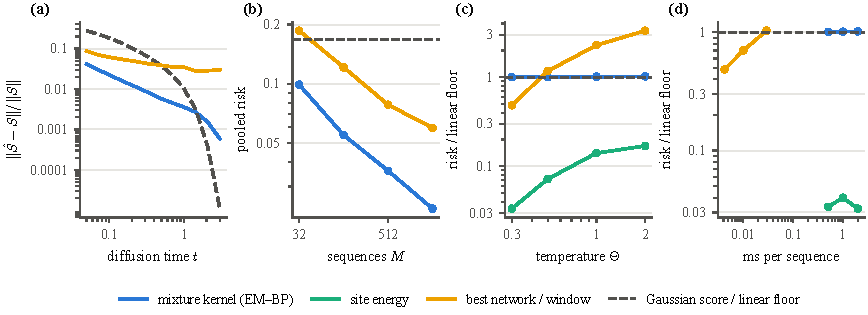
\includegraphics[width=\textwidth]{ff-summary.pdf}
\caption{The headline in one picture. (a,~b) Part I, the paper's chain: error per noise level at $M=2048$, and error against $M$. The
learned kernel (blue) beats the best network (yellow; trained on clean sequences) at every level and size, and the Gaussian score
(dashed) except at the highest noise levels in (a), $t\gtrsim2$. (c) Part II, the $\phi^4$ field: risk divided by the linear
baseline (dashed) across temperature at $M=2048$. The site energy (green) is far below it, the paper's mixture kernel (blue) sits
on it, the window network (yellow; DSM, i.e.\ trained with clean targets) rises above it when hot. (d) The same ratio against
inference time (ms per sequence, 8 threads, largest network variants) on three lattice spacings at $\Theta=0.3$.}
\label{fig:summary}
\end{figure}

\textbf{The paper (12 October).} The draft was rewritten to follow Jérôme's and Marc's note: it opens with the structural message (learn the
local law, infer globally) and a summary figure; states everything for a general Markov kernel, with the linear chain as the first
example and the $\phi^4$ field as the second; has a Gaussian sanity-check section (BP with Gaussian messages is the linear score
and the Kalman smoother); presents the Fisher/Hermite theory as a supporting subsection rather than the headline; gives the field its
own section with the temperature sweep, the scoreboard, the physical reading of the fitted kernel, runtime and speciation; and has a
cost section with the coarse grid and the reasons not to use Fourier modes. Every number in it is generated from the frozen outputs, and
the consistency checks and the independent audit pass. It is 39 pages against an 8-page body limit, on purpose: the cut is yours, and
\path{docs/PAPER_REWRITE_2026-10-12.md} lists what to keep (summary, method, Gaussian sanity, per-level gain, sample efficiency, field
sweep, accuracy against cost) and what can go to the appendix.

\textbf{An internal audit (9 October)} re-derived the numbers in the registry, the reports and the question ledger from the frozen
files. It changed no existing verdict, but it found three runs never frozen (now frozen), gave first verdicts to predictions never
read (one falsified, one unresolved), replaced numbers that had been quoted from unfrozen laptop runs, and flagged speciation as not
addressed (hence E50). The corrections are applied, each logged in its registry file; this document uses the corrected numbers.

\textbf{Drafted in the paper, waiting for your approval.}
\begin{enumerate}[leftmargin=1.6em]
\item The framing Jérôme suggested on 30 September (a general Markov kernel; the linear chain first, the field second) and the field
in the body rather than the appendix, which is what makes the paper long.
\item The information panel (Q10) is re-plotted in cumulant coordinates ($\kappa_2$, $\kappa_4$); the alternative was to keep $\beta$
and drop the label ``fourth order''.
\item The figures: the summary figure plus the key ones named above; the rest are candidates for the appendix.
\end{enumerate}

\textbf{Yours to do.} The reply to Jérôme \emph{and Marc}, this week (12--16 October); tell Jérôme the Milan date once it is confirmed.

\medskip
{\footnotesize\color{gray}\raggedright Sources: \path{experiments/registry/E*.json} (hypotheses, predictions, outcomes, corrections)
and the frozen outputs they list; \path{reports/field-laboratory-2026-10-01.pdf} (full detail);
\path{docs/JEROME_CALL_2026-09-25.md} (the question ledger). Branch \path{claude/phi4-field-2026-10-01}.\par}

\end{document}
